\documentclass[12pt]{article}

% 使用ctex包来支持中文
\usepackage[UTF8,heading=false,scheme=plain]{ctex}

% 设置中文字体
\setCJKmainfont{STSong}

\usepackage{graphicx} % 用于包含图像
\usepackage{amsmath} % 数学内容支持
\usepackage{geometry}
\geometry{left=3cm,right=3cm,top=2.5cm,bottom=2.5cm}
\usepackage{hyperref} % 用于超链接
\usepackage{parskip} % 用于段落间距,取消首行缩进
\usepackage{ulem} % 用于下划线
\usepackage{titlesec} % 用于设置标题格式
\usepackage{xcolor} % 用于代码高亮
\usepackage{listings} % 用于代码显示
\usepackage{enumitem} % 用于设置列表格式

% 设置段落格式
\setlength{\parindent}{0pt} % 取消首行缩进
\setlength{\parskip}{6pt} % 段落之间的间距
\setlength{\leftskip}{0pt} % 设置正文左边距为0

% 设置标题格式
\titleformat{\section}[hang]
{\normalfont\Large\bfseries}{\thesection}{1em}{}
\titlespacing{\section}
{0pt}{3.5ex plus 1ex minus .2ex}{2.3ex plus .2ex}

\titleformat{\subsection}[hang]
{\normalfont\large\bfseries}{\thesubsection}{1em}{}
\titlespacing{\subsection}
{0pt}{2.5ex plus 1ex minus .2ex}{1.5ex plus .2ex}

\titleformat{\subsubsection}[hang]
{\normalfont\normalsize\bfseries}{\thesubsubsection}{1em}{}
\titlespacing{\subsubsection}
{0pt}{2ex plus 1ex minus .2ex}{1ex plus .2ex}

% 设置列表格式
\setlist[itemize]{left=0pt, label={$\bullet$}, leftmargin=2em, itemsep=1pt}
\setlist[enumerate]{left=0pt, leftmargin=2em, itemsep=1pt}

% 设置MATLAB代码环境
\definecolor{codegreen}{rgb}{0,0.6,0}
\definecolor{codegray}{rgb}{0.5,0.5,0.5}
\definecolor{codepurple}{rgb}{0.58,0,0.82}
\definecolor{backcolour}{rgb}{0.95,0.95,0.92}

\lstdefinestyle{mystyle}{
    backgroundcolor=\color{backcolour},   
    commentstyle=\color{codegreen},
    keywordstyle=\color{magenta},
    numberstyle=\tiny\color{codegray},
    stringstyle=\color{codepurple},
    basicstyle=\ttfamily\footnotesize,
    breakatwhitespace=false,         
    breaklines=true,                 
    captionpos=b,                    
    keepspaces=true,                 
    numbers=left,                    
    numbersep=5pt,                  
    showspaces=false,                
    showstringspaces=false,
    showtabs=false,                  
    tabsize=2
}

\lstset{style=mystyle}

% 定义MATLAB语言
\lstdefinelanguage{MATLAB}{
  keywords={break,case,catch,continue,else,elseif,end,for,function,global,if,otherwise,persistent,return,switch,try,while},
  keywordstyle=\color{blue},
  identifierstyle=\color{black},
  sensitive=false,
  comment=[l]\%,
  morecomment=[s]{\%\{}{\%\}},
  commentstyle=\color{codegreen},
  stringstyle=\color{magenta},
  string=[b]',
  basicstyle=\ttfamily\footnotesize,
  moredelim=[il][\textcolor{magenta}]{\$},
  moredelim=[is][\textcolor{magenta}]{\%\%}{\%\%},
  morekeywords={abs,sin,cos,plot,exp,log,ones,zeros,linspace,meshgrid,figure,hold,xlabel,ylabel,title,grid},
  otherkeywords={.,\,,;,-,+,*,/,^},
  alsoletter={.,\,,;,-,+,*,/,^}
}

% 重定义标题格式
\renewcommand{\maketitle}{
    \begin{titlepage}
        \begin{center}
            \vspace*{0cm}
            
            {\huge \kaishu \textbf{电子科技大学格拉斯哥海南学院}}
            
            \vspace{0.5cm}
            {\Large \textbf{UOG-UESTC Joint School of UESTC}}
            
            \vspace{4cm}
            
            {\Huge \kaishu \textbf{标 准 实 验 报 告}}
            
            \vspace{0.5cm}
            {\Large \textbf{Lab Report}}
            
            \vspace{4cm}
            
            \begin{center}
            \begin{tabular}{rc}
                \kaishu (实验)课程名称: & \kaishu 信号与系统 \\[0.5cm]
                (LAB) Course Name: & Signals and Systems
            \end{tabular}
            \end{center}
            
            \vfill
            
            {\large \kaishu 电子科技大学教务处制表}
        \end{center}
    \end{titlepage}
    
    % 第二页的内容
    \noindent
    \begin{tabular}{ll@{\hspace{4cm}}ll}
        \textbf{Student Name:} & ABC & \textbf{Student No.:} & 2099999999 \\[0.5cm]
        \textbf{Instructor:} & 邬震宇 & \textbf{Date:} & 2025/3/22 \\[0.5cm]
        \textbf{Location:} & Gensokyo
    \end{tabular}
    
    \vspace{1cm}
}

% 文档开始
\begin{document}

\maketitle

\section{Laboratory Name}
Signals and Systems

\section{Project Name}
Represent signals using MATLAB

\section{lab Hours}
4 hours

\section{Theoretical Background}
\begin{enumerate}[leftmargin=2em]
    \item The basic concepts of signals and systems arise in a variety of contexts, from engineering design to financial analysis. In this lab1, you will learn how to represent, manipulate, and analyze basic signals and systems in MATLAB.
    \item Some basic MATLAB commands for representing signals include: zeros, ones, cos, sin, exp, real, imag, abs, angle, linspace, plot, stem, subplot, xlabel, ylabel, title.
    \item Some useful commands in Symbolic Math Toolbox are as: sym, subs, ezplot.
\end{enumerate}


\section{Objectives}
\begin{enumerate}
    \item Familiarize with some basic MATLAB commands to represent and plot continuous-time and discrete-time signals.
    \item Use MATLAB to perform operations on signals, including transformations.
    \item Use MATLAB to analyze signal periodicity.
    \item Use MATLAB to calculate signal energy and power.
\end{enumerate}

\section{Description}
The following exercises are from the book, "John R.Buck, Michael M. Daniel, Andrew C. Singer. Computer Exploration in Signals and Systems —— Using MATLAB."

\section{Required Equipment}
Computer, MATLAB

\section{Procedure, Data Analysis, Results, and Conclusion}

\subsection{1.2 (d)}
\subsubsection{Codes}
\begin{lstlisting}[language=MATLAB]
t = linspace(-5,5,1000);
x = exp(-t).*cos(2*pi*t);
plot(t,x,'LineWidth',1.5);
grid on;
xlabel('t');
ylabel('x(t)');
title('x(t)=e^{-t}cos(2\pit)');
\end{lstlisting}

\subsubsection{Figure}
\begin{figure}[h]
    \centering
    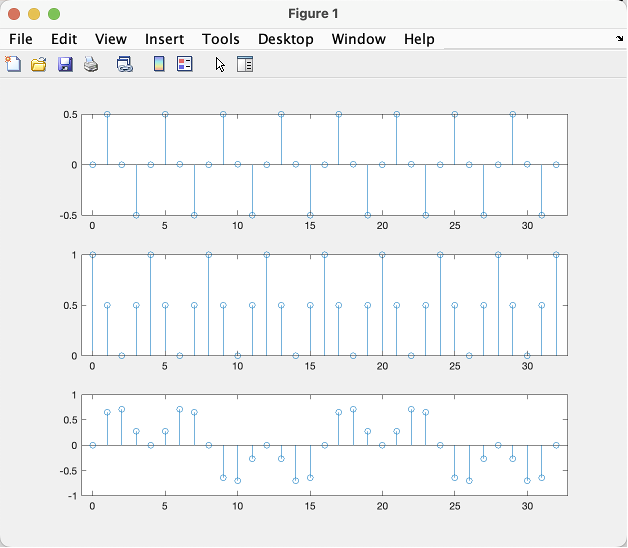
\includegraphics[width=0.5\textwidth]{imgs/1-2b.png}
    \caption{1.2 (d)}
    \label{fig_1.2d}
\end{figure}

\subsubsection{Explanations}

Add your content here.

\section{Summary and Comments}
After completing this experiment,

\section{Suggestions for This Experiment}
None.

\section*{}  % 创建一个无标题的section
\vspace{1cm}
\begin{flushright}
\begin{tabular}{r@{\hspace{1cm}}l}
Score: & \hspace{3cm} \\[1cm]
Instructor: & \hspace{3cm}
\end{tabular}
\end{flushright}

\end{document}